% =====================================================================
% CS769 Interim Project Presentation
% Multi-objective Optimisation for Multilingual Tokenization
% Compile on Overleaf with pdfLaTeX (Menu > Compiler > pdfLaTeX).
% Course format: 5 slides (excluding title), 4 min talk + 1 min questions.
% Speaker notes for each slide are in comments above it.
% The chart on slide 4 has its numbers written into this file, so no
% results.csv needs to be uploaded.
% =====================================================================
\documentclass[aspectratio=169,10pt]{beamer}

% ========== Fonts ==========
\usepackage[T1]{fontenc}
\usepackage[scaled]{helvet}
\usefonttheme[onlymath]{serif}

% ========== Packages ==========
\usepackage{amsmath,amssymb}
\usepackage{booktabs,tabularx,array}
\usepackage[most]{tcolorbox}
\usepackage{tikz}
\usetikzlibrary{arrows.meta,positioning,calc}
\usepackage{pgfplots}
\pgfplotsset{compat=1.18}

% ========== Colours ==========
\definecolor{iitbblue}{HTML}{0B3D91}
\definecolor{accent}{HTML}{D9622B}
\definecolor{ink}{HTML}{1F2933}
\definecolor{muted}{HTML}{6B7280}
\definecolor{soft}{HTML}{EEF2F8}
\definecolor{good}{HTML}{2E7D32}

% ========== Beamer look ==========
\setbeamersize{text margin left=0.8cm,text margin right=0.8cm}
\setbeamercolor{normal text}{fg=ink}
\setbeamercolor{structure}{fg=iitbblue}
\setbeamercolor{frametitle}{fg=iitbblue}
\setbeamercolor{alerted text}{fg=accent}
\setbeamerfont{frametitle}{size=\Large,series=\bfseries}
\setbeamerfont{title}{size=\LARGE,series=\bfseries}
\setbeamerfont{subtitle}{size=\large}
\setbeamertemplate{navigation symbols}{}
\setbeamertemplate{itemize item}{\color{accent}\scriptsize$\blacktriangleright$}
\setbeamertemplate{itemize subitem}{\color{muted}\scriptsize$\bullet$}
\setbeamertemplate{enumerate item}{\color{accent}\bfseries\insertenumlabel.}
\setlength{\leftmargini}{1.1em}

\setbeamertemplate{frametitle}{%
  \nointerlineskip\vskip0.3cm%
  \begin{beamercolorbox}[wd=\paperwidth,leftskip=0.8cm,rightskip=0.8cm]{frametitle}%
    \usebeamerfont{frametitle}\insertframetitle\par\vskip2pt%
    {\color{accent}\rule{1.4cm}{2pt}}%
  \end{beamercolorbox}%
  \vskip-2pt%
}

\setbeamertemplate{footline}{%
  \hbox to \paperwidth{%
    \hskip0.8cm{\color{muted}\tiny Group 30 \textbullet{} Multi-objective optimisation for multilingual tokenization \textbullet{} CS769 interim presentation}%
    \hfill{\color{muted}\tiny\insertframenumber/\inserttotalframenumber}\hskip0.8cm}%
  \vskip0.2cm}

\setbeamertemplate{title page}{%
  \vfill
  {\color{accent}\rule{2cm}{3pt}}\par\vskip0.4cm
  {\usebeamerfont{title}\color{iitbblue}\inserttitle\par}
  \vskip0.25cm
  {\usebeamerfont{subtitle}\color{ink}\insertsubtitle\par}
  \vskip0.7cm
  {\small\color{ink}\insertauthor\par}
  \vskip0.1cm
  {\footnotesize\color{muted}\insertinstitute\par}
  \vskip0.1cm
  {\footnotesize\color{muted}\insertdate\par}
  \vfill
}

% ========== Helpers ==========
\newtcolorbox{keybox}[1][]{enhanced,colback=soft,colframe=soft,boxrule=0pt,arc=3pt,
  left=6pt,right=6pt,top=3pt,bottom=3pt,fontupper=\small\raggedright,#1}
\newtcolorbox{accentbox}[1][]{enhanced,colback=white,colframe=accent,boxrule=0.8pt,arc=3pt,
  left=6pt,right=6pt,top=3pt,bottom=3pt,fontupper=\small\raggedright,#1}
\newtcolorbox{placeholder}[1][]{enhanced,colback=white,colframe=white,
  borderline={0.6pt}{0pt}{muted,dashed},arc=3pt,left=8pt,right=8pt,top=6pt,bottom=6pt,
  fontupper=\footnotesize\color{muted},halign=center,valign=center,#1}
\newcommand{\refnote}[1]{{\color{muted}\scriptsize[#1]}}
\newcommand{\done}{\textcolor{good}{$\checkmark$}}
\newcommand{\wip}{\textcolor{accent}{$\circ$}}

% ========== Title ==========
\title{Multi-objective Optimisation for Multilingual Tokenization}
\subtitle{Tracing the compression--parity--morphology front of vocabulary learning}
\author{Vaibhav Rathore {\color{muted}\footnotesize(25D1387)} \quad\textbullet\quad Siddhant Gole {\color{muted}\footnotesize(26D1384)}}
\institute{Group 30 \textbullet{} CS769 Optimization in Machine Learning \textbullet{} IIT Bombay \textbullet{} Interim project presentation\\[2pt]\texttt{\{25d1387, 26d1384\}@iitb.ac.in}}
\date{October 2026}

\begin{document}

% =====================================================================
\begin{frame}[plain,noframenumbering]
  \titlepage
\end{frame}

% =====================================================================
% SLIDE 1: Problem and motivation   (about 45 s)
% Tokenizers are trained by frequency, so dominant languages get most merges
% and everyone else pays more tokens for the same content. Word-level
% fertility hides this: Sanskrit words carry far more content than Hindi
% words, so we measure tokens per parallel sentence (the same sentence in
% every language; bytes would not work across scripts, because a Devanagari
% or Gujarati character is 3 bytes and a Latin one is 1). Compression, parity
% and morphology pull in different directions, and every existing tokenizer
% silently picks one trade-off. We ask whether we can treat this as vector
% optimisation and trace the whole front.
% =====================================================================
\begin{frame}{Problem and motivation}
\begin{columns}[T,onlytextwidth]
\begin{column}{0.55\textwidth}
\begin{itemize}\setlength{\itemsep}{2pt}
  \item Frequency-driven BPE gives its merges to dominant languages, so the same content can cost up to $15\times$ more tokens \refnote{Petrov et al., 2023}.
  \item Inference cost, latency and lost context fall on exactly these languages.
  \item Word fertility hides the gap: parallel hin/san sentences have similar length (68.2 vs.\ 67.6 chars) but 12.97 vs.\ 8.90 words \refnote{Samas\={a}mayik, 2026}. We measure \textbf{tokens per parallel sentence}.
  \item Compression, parity and morphology conflict \refnote{SuTRA, 2026}, yet each tokenizer fixes one trade-off implicitly.
\end{itemize}
\end{column}
\begin{column}{0.42\textwidth}
\centering
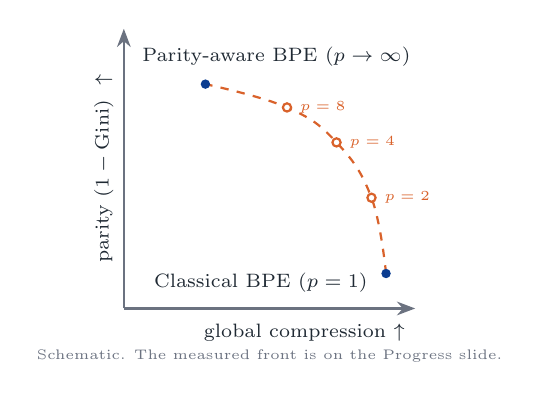
\begin{tikzpicture}[scale=0.74,>=Stealth]
  \draw[->,thick,draw=muted] (0,0) -- (5,0)
    node[anchor=north east,font=\scriptsize,text=ink,yshift=-2pt]{global compression $\uparrow$};
  \draw[->,thick,draw=muted] (0,0) -- (0,4.8)
    node[midway,above,rotate=90,font=\scriptsize,text=ink]{parity $(1-\mathrm{Gini})\ \uparrow$};
  \draw[accent,thick,dashed] plot[smooth,tension=0.7] coordinates
    {(4.5,0.6) (4.25,1.9) (3.65,2.85) (2.8,3.45) (1.4,3.85)};
  \foreach \x/\y/\l in {4.25/1.9/2, 3.65/2.85/4, 2.8/3.45/8}{
    \draw[accent,thick,fill=white] (\x,\y) circle (2pt)
      node[right,font=\tiny,text=accent,xshift=1pt]{$p=\l$};
  }
  \fill[iitbblue] (4.5,0.6) circle (2.3pt);
  \node[font=\scriptsize,anchor=east,text=ink] at (4.35,0.45) {Classical BPE ($p=1$)};
  \fill[iitbblue] (1.4,3.85) circle (2.3pt);
  \node[font=\scriptsize,anchor=south west,text=ink] at (0.15,3.98) {Parity-aware BPE ($p\to\infty$)};
  \node[font=\tiny,text=muted,anchor=north] at (2.5,-0.55)
    {Schematic. The measured front is on the Progress slide.};
\end{tikzpicture}
\end{column}
\end{columns}
\vskip2pt
\begin{accentbox}
\textbf{Research question.} Can we cast vocabulary learning as vector optimisation and trace the full trade-off front, instead of committing to one implicit scalarisation?
\end{accentbox}
\end{frame}

% =====================================================================
% SLIDE 2: Related work   (about 45 s)
% Zouhar et al. show BPE is greedy submodular maximisation of one objective.
% Parity-aware BPE replaces it with a max-min rule, which controls only the
% worst language; a 2026 study finds the English gap still widens with
% vocabulary size. The Indic study allocates cluster budgets with a heuristic
% and finds Dravidian languages lose. We show the first two are the two ends
% of one family and replace the heuristic allocation with a KKT solution
% over script clusters (Devanagari, Gujarati, Latin).
% =====================================================================
\begin{frame}{Related work and how we differ}
\small
\renewcommand{\arraystretch}{1.2}
\begin{tabularx}{\textwidth}{@{}>{\raggedright\arraybackslash}p{3.7cm}>{\raggedright\arraybackslash}X>{\raggedright\arraybackslash}X@{}}
\toprule
\textbf{Work} & \textbf{What it optimises} & \textbf{Gap for our goal}\\
\midrule
Zouhar et al.\newline{\color{muted}\footnotesize ACL Findings 2023} &
BPE as submodular maximisation of tokens saved; greedy has a curvature-dependent guarantee. &
One objective (global compression); no per-language cost.\\
Parity-aware BPE\newline{\color{muted}\footnotesize Foroutan et al., ACL 2026} &
Max--min rule: each merge targets the worst-compressed language. &
Only the worst case; English gap widens 36\% from 45k to 135k vocabulary \refnote{Equity w/ Efficiency, 2026}.\\
Indic tokenization study\newline{\color{muted}\footnotesize Brahma, Karthika et al., 2025} &
17 Indic languages; cluster budgets set by a vocabulary-union proportion. &
Heuristic allocation; 3 of 4 Dravidian languages lose fertility under family clustering.\\
\bottomrule
\end{tabularx}
\vskip6pt
\begin{accentbox}
\textbf{Our position.} Classical and Parity-aware BPE are two scalarisations of one vector problem. We define a power-mean family containing both, trace the front between them, and replace heuristic budgets with a convex program over script clusters, solved through KKT.
\end{accentbox}
\end{frame}

% =====================================================================
% SLIDE 3: Dataset and approach   (about 60 s, the main slide)
% Three Indic languages (Hindi, Marathi, Gujarati) with English as the
% dominant-language anchor. All three have SuTRA gold morpheme data, so every
% Indic language is scored on all three axes. Clusters are by script:
% Devanagari (hin + mar), Gujarati, Latin. English gets 4x the training text
% of the others, to play the dominant language. Cost t is tokens per parallel
% sentence: FLORES dev measures it during training, FLORES devtest gives the
% reported numbers. At the token level we minimise a power mean of
% per-language token cost. Its first-order greedy step is a weighted pair count with
% weights t^(p-1): p = 1 gives exactly classical BPE, and as p grows the
% weight concentrates on the worst language, which is the subgradient of the
% max and gives Parity-aware BPE. At the allocation level the composition
% rule makes the budget problem convex, and KKT gives a water-filling
% solution we compute by bisection.
% =====================================================================
\begin{frame}{Dataset and approach}
\begin{columns}[T,onlytextwidth]
\begin{column}{0.29\textwidth}
\footnotesize
\textbf{\color{iitbblue}\small Data}
\begin{itemize}\setlength{\itemsep}{3pt}
  \item \textbf{Languages:} hin, mar, guj; eng as anchor.
  \item \textbf{Script clusters:} Devanagari (hin, mar), Gujarati (guj), Latin (eng).
  \item \textbf{Training:} Sangraha, 20M characters per language; eng $4\times$ (80M).
  \item \textbf{Parity:} FLORES-200, parallel in all four; dev steers training, devtest scores.
  \item \textbf{Morphology:} SuTRA gold segmentation for hin, mar, guj.
  \item \textbf{Downstream:} hin--mar MT (chrF++), CSTT technical terms.
\end{itemize}
\end{column}
\begin{column}{0.68\textwidth}
\begin{keybox}
\textbf{\color{iitbblue}(1) Token level: $p$-fair BPE.} $t_\ell$: tokens per parallel sentence in language $\ell$; $\pi_\ell$: share of training text.
\vskip-6pt
\[
\min\nolimits_{|V|\le K}\;\Big(\textstyle\sum_\ell \pi_\ell\, t_\ell(V)^{p}\Big)^{1/p}+\lambda\,\beta(V)
\]
\vskip-4pt
Greedy merge: $\arg\max_{(a,b)}\sum_\ell t_\ell^{\,p-1}c_\ell(a,b)-\lambda\,\beta(a,b)$
{\color{muted}\footnotesize($c_\ell$: pair count; $\beta$: morpheme-boundary crossings)}\\[3pt]
$p=1$: \textbf{classical BPE}. \; $p\to\infty$: subgradient of $\max_\ell t_\ell$ picks the worst language, \textbf{Parity-aware BPE} (Lec.~14).
\end{keybox}
\vskip-2pt
\begin{keybox}
\textbf{\color{iitbblue}(2) Allocation level: budgets via KKT.} Script-cluster budgets $k_c$, fitted $t_c(k)=a_c k^{-b_c}+d_c$.
\vskip-6pt
\[
\min\nolimits_{k\ge 0,\;\sum_c k_c=K}\;\textstyle\sum_c \pi_c\, t_c(k_c)^{p}
\]
\vskip-4pt
Convex for $p\ge1$ (composition rule, Lec.~10). KKT (Lec.~16--17): $p\,\pi_c\,t_c^{\,p-1}|t_c'(k_c)|=\mu$ for $k_c>0$, bisection on $\mu$ (water-filling).
\end{keybox}
\end{column}
\end{columns}
\end{frame}

% =====================================================================
% SLIDE 4: Progress so far   (about 40 s)
% Everything on the status list is done. One trainer covers classical,
% Parity-aware and p-fair BPE; it is exact (checked against brute force) and
% takes about 15 s per 32k tokenizer. The chart is the measured front: each
% point is the mean of 5 different samples of training text, bars are one
% standard deviation (they are smaller than the markers for most points).
% Reading the chart: top right is classical BPE (best compression, least
% fair), bottom left is Parity-aware (fairest, 4% worse compression), and
% raising p walks down the curve. Every step lowered both Gini and
% compression in 5 of 5 samples. The orange squares are the hybrid baseline
% from the Parity-aware paper (classical merges first, then parity merges):
% it lies on the same curve, so p-fair matches it and does not beat it.
% Parity-aware and hybrid are our own implementation of the paper's rules.
% Chart data: results_errorbars/results_errorbars.csv from error_bars.py.
% =====================================================================
\begin{frame}{Progress so far}
\begin{columns}[T,onlytextwidth]
\begin{column}{0.5\textwidth}
\textbf{\color{iitbblue}Status}
\begin{itemize}\setlength{\itemsep}{2pt}
  \item[\done] Literature review and positioning.
  \item[\done] Unified formulation; $p=1$ is classical BPE exactly.
  \item[\done] Convexity of budget allocation; KKT solution.
  \item[\done] Exact, fast trainer: $\sim$15\,s per 32k tokenizer.
  \item[\done] Front traced for $p=1,\dots,32,\infty$, with hybrid baseline and error bars.
\end{itemize}
\vskip2pt
\begin{keybox}[fontupper=\footnotesize\raggedright]
\textbf{Result so far} (32k, eng $4\times$). Classical BPE charges Hindi 21\% more tokens than English per sentence. Each step up in $p$ lowers Gini and compression, in 5 of 5 samples; $p=8$ cuts Gini by 40\% for 0.6\% of compression. $p$-fair matches the hybrid baseline; it does not beat it.
\end{keybox}
\end{column}
\begin{column}{0.46\textwidth}
\centering
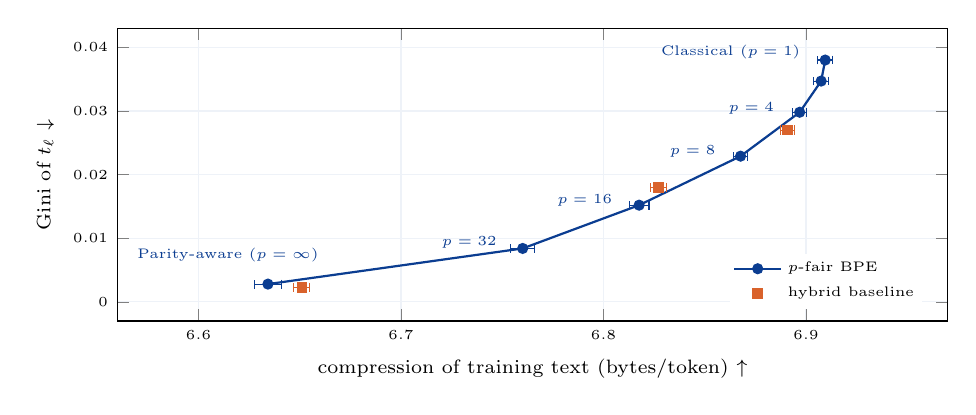
\begin{tikzpicture}
\begin{axis}[
  width=\linewidth, height=5.3cm,
  xlabel={compression of training text (bytes/token) $\uparrow$},
  ylabel={Gini of $t_\ell$ $\downarrow$},
  label style={font=\scriptsize}, tick label style={font=\tiny},
  grid=major, grid style={draw=soft},
  xmin=6.56, xmax=6.97, ymin=-0.003, ymax=0.043,
  xtick={6.6,6.7,6.8,6.9}, ytick={0,0.01,0.02,0.03,0.04},
  scaled y ticks=false,
  yticklabel style={/pgf/number format/fixed,/pgf/number format/precision=2},
  legend style={font=\tiny, at={(0.97,0.04)}, anchor=south east, draw=none, fill=white, inner sep=1pt},
  legend cell align=left]
% p-fair BPE: mean of 5 samples, +- one standard deviation (compression, Gini)
\addplot[mark=*, mark size=1.6pt, color=iitbblue, thick,
  error bars/.cd, x dir=both, x explicit, y dir=both, y explicit]
  coordinates {
    (6.9095,0.0380) +- (0.0036,0.0002)
    (6.9075,0.0347) +- (0.0036,0.0002)
    (6.8969,0.0298) +- (0.0035,0.0002)
    (6.8677,0.0229) +- (0.0036,0.0002)
    (6.8176,0.0152) +- (0.0049,0.0002)
    (6.7601,0.0084) +- (0.0059,0.0001)
    (6.6343,0.0028) +- (0.0067,0.0004)
  };
% hybrid baseline: 50%, 75% and 90% of the merges classical, the rest Parity-aware
\addplot[only marks, mark=square*, mark size=1.7pt, color=accent,
  error bars/.cd, x dir=both, x explicit, y dir=both, y explicit]
  coordinates {
    (6.6510,0.0023) +- (0.0039,0.0004)
    (6.8271,0.0180) +- (0.0039,0.0005)
    (6.8908,0.0270) +- (0.0034,0.0002)
  };
\legend{$p$-fair BPE, hybrid baseline}
\node[font=\tiny, text=iitbblue, anchor=east] at (axis cs:6.9020,0.0392) {Classical ($p=1$)};
\node[font=\tiny, text=iitbblue, anchor=east] at (axis cs:6.8890,0.0304) {$p=4$};
\node[font=\tiny, text=iitbblue, anchor=east] at (axis cs:6.8600,0.0236) {$p=8$};
\node[font=\tiny, text=iitbblue, anchor=east] at (axis cs:6.8090,0.0160) {$p=16$};
\node[font=\tiny, text=iitbblue, anchor=east] at (axis cs:6.7520,0.0094) {$p=32$};
\node[font=\tiny, text=iitbblue, anchor=south west] at (axis cs:6.5650,0.0048) {Parity-aware ($p=\infty$)};
\end{axis}
\end{tikzpicture}\\[-2pt]
{\tiny\color{muted}Mean $\pm$ s.d.\ over 5 training samples; Gini on FLORES-200 devtest.\\[-1pt]
Parity-aware and hybrid: our implementation of the published rules.\par}
\end{column}
\end{columns}
\end{frame}

% =====================================================================
% SLIDE 5: Next steps and challenges   (about 40 s)
% The p sweep is done, so the next axis is morphology: add the lambda
% penalty and report hypervolume. Scaling: classical Gini is the same at 32k
% and 64k (0.038, single run each), so we extend to 128k. Then KKT allocation
% against the heuristics over script clusters, and downstream checks with
% Hindi-Marathi MT and technical terms. What we learned the hard way: p-fair
% and the hybrid schedule give the same front, so any advantage has to come
% from lambda or allocation; measuring cost per byte reverses the result,
% because 3-byte Indic scripts look cheap and the parity methods then give
% their merges to English; and with equal data classical BPE is already
% close to parity (Gini 0.019), so the gap comes from the 4x English anchor.
% =====================================================================
\begin{frame}{Next steps and challenges}
\begin{columns}[T,onlytextwidth]
\begin{column}{0.53\textwidth}
\textbf{\color{iitbblue}Plan to final submission}
\begin{enumerate}\setlength{\itemsep}{4pt}
  \item \textbf{Morphology:} add the $\lambda$ penalty with SuTRA boundaries; report hypervolume.
  \item \textbf{Scaling:} Gini is unchanged from 32k to 64k (0.038); extend to 128k.
  \item \textbf{Allocation} (script clusters): KKT vs.\ union-proportion vs.\ uniform budgets.
  \item \textbf{Extrinsic:} hin--mar MT (chrF++), fertility on CSTT terms.
  \item \textbf{Extension:} $p$-fair Unigram pruning.
\end{enumerate}
\end{column}
\begin{column}{0.44\textwidth}
\textbf{\color{iitbblue}Challenges}
\begin{itemize}\setlength{\itemsep}{4pt}
  \item $p$-fair and the hybrid schedule trace the same front; an advantage must come from $\lambda$ or allocation.
  \item The cost unit decides the outcome: per byte, 3-byte Indic scripts look cheap and parity favours English.
  \item With equal data, classical BPE is near parity (Gini 0.019); the gap comes from the eng anchor.
  \item Morphology need not track downstream quality, so we keep it as a separate axis.
\end{itemize}
\end{column}
\end{columns}
\vskip10pt
% \begin{accentbox}
% \textbf{Target.} A workshop paper on tokenization or optimisation for ML, with the course report as its first draft.
% \end{accentbox}
\end{frame}

\end{document}